%tikz
\usepackage{tikz}
\usetikzlibrary{knots, cd, calc}



\newcommand{\coxtwothreethree}{%
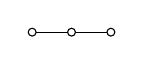
\begin{tikzpicture}[scale=0.5]
\draw (0, 0) circle (0.1);
\draw (1, 0) circle (0.1);
\draw (2, 0) circle (0.1);
\draw (0.1, 0) -- (0.9, 0);
\draw (1.1, 0) -- (1.9, 0);
\end{tikzpicture}}

\newcommand{\coxthreethreethree}{%
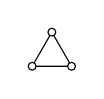
\begin{tikzpicture}[scale = 0.5]
\draw (0, 0) -- (60:1) -- (1, 0) -- (0, 0);
\draw[fill = white] (0, 0) circle (0.1);
\draw[fill = white] (60:1) circle (0.1);
\draw[fill = white] (1, 0) circle (0.1);
\end{tikzpicture}}

\newcommand{\coxthreethreethreetype}[1]{%
\begin{tikzpicture}[scale = 0.5]
\draw (0, 0) -- (60:1) -- (1, 0) -- (0, 0);
\draw[fill = white] (0, 0) circle (0.1);
\draw[fill = white] (60:1) circle (0.1);
\draw[fill = white] (1, 0) circle (0.1);
\node at (0.5, 0.2) {\tiny{#1}};
\end{tikzpicture}}

\newcommand{\coxathreetype}[1]{%
\begin{tikzpicture}[scale=0.5]
\draw (0, 0) circle (0.1);
\draw (1, 0) circle (0.1);
\draw (2, 0) circle (0.1);
\draw (0.1, 0) -- (0.9, 0);
\draw (1.1, 0) -- (1.9, 0);

\node at (0.5, 0.2) {\tiny{#1}};
\end{tikzpicture}}

\newcommand{\coxathreetypedouble}[2]{%
\begin{tikzpicture}[scale=0.5]
\draw (0, 0) circle (0.1);
\draw (1, 0) circle (0.1);
\draw (2, 0) circle (0.1);
\draw (0.1, 0) -- (0.9, 0);
\draw (1.1, 0) -- (1.9, 0);

\node at (0.5, 0.2) {\tiny{#1}};
\node at (1.5, 0.2) {\tiny{#2}};
\end{tikzpicture}}

\newcommand{\coxfourthreethree}{%
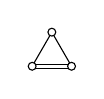
\begin{tikzpicture}[scale = 0.5]
\draw (0, 0) -- (60:1) -- (1, 0);
\draw (0, 0.05) -- (1, 0.05);
\draw (0, -0.05) -- (1, -0.05);
\draw[fill = white] (0, 0) circle (0.1);
\draw[fill = white] (60:1) circle (0.1);
\draw[fill = white] (1, 0) circle (0.1);
\end{tikzpicture}
}
